% Options for packages loaded elsewhere
\PassOptionsToPackage{unicode,linktoc=all,pdfwindowui}{hyperref}
\PassOptionsToPackage{hyphens}{url}
\PassOptionsToPackage{dvipsnames,svgnames,x11names}{xcolor}
%
\documentclass[
  12pt,
]{article}
\usepackage{amsmath,amssymb}
\usepackage{lmodern}
\usepackage{iftex}
\ifPDFTeX
  \usepackage[T1]{fontenc}
  \usepackage[utf8]{inputenc}
  \usepackage{textcomp} % provide euro and other symbols
\else % if luatex or xetex
  \usepackage{unicode-math}
  \defaultfontfeatures{Scale=MatchLowercase}
  \defaultfontfeatures[\rmfamily]{Ligatures=TeX,Scale=1}
\fi
% Use upquote if available, for straight quotes in verbatim environments
\IfFileExists{upquote.sty}{\usepackage{upquote}}{}
\IfFileExists{microtype.sty}{% use microtype if available
  \usepackage[]{microtype}
  \UseMicrotypeSet[protrusion]{basicmath} % disable protrusion for tt fonts
}{}
\makeatletter
\@ifundefined{KOMAClassName}{% if non-KOMA class
  \IfFileExists{parskip.sty}{%
    \usepackage{parskip}
  }{% else
    \setlength{\parindent}{0pt}
    \setlength{\parskip}{6pt plus 2pt minus 1pt}}
}{% if KOMA class
  \KOMAoptions{parskip=half}}
\makeatother
\usepackage{xcolor}
\usepackage[margin=1.0in]{geometry}
\usepackage{color}
\usepackage{fancyvrb}
\newcommand{\VerbBar}{|}
\newcommand{\VERB}{\Verb[commandchars=\\\{\}]}
\DefineVerbatimEnvironment{Highlighting}{Verbatim}{commandchars=\\\{\}}
% Add ',fontsize=\small' for more characters per line
\usepackage{framed}
\definecolor{shadecolor}{RGB}{248,248,248}
\newenvironment{Shaded}{\begin{snugshade}}{\end{snugshade}}
\newcommand{\AlertTok}[1]{\textcolor[rgb]{0.94,0.16,0.16}{#1}}
\newcommand{\AnnotationTok}[1]{\textcolor[rgb]{0.56,0.35,0.01}{\textbf{\textit{#1}}}}
\newcommand{\AttributeTok}[1]{\textcolor[rgb]{0.77,0.63,0.00}{#1}}
\newcommand{\BaseNTok}[1]{\textcolor[rgb]{0.00,0.00,0.81}{#1}}
\newcommand{\BuiltInTok}[1]{#1}
\newcommand{\CharTok}[1]{\textcolor[rgb]{0.31,0.60,0.02}{#1}}
\newcommand{\CommentTok}[1]{\textcolor[rgb]{0.56,0.35,0.01}{\textit{#1}}}
\newcommand{\CommentVarTok}[1]{\textcolor[rgb]{0.56,0.35,0.01}{\textbf{\textit{#1}}}}
\newcommand{\ConstantTok}[1]{\textcolor[rgb]{0.00,0.00,0.00}{#1}}
\newcommand{\ControlFlowTok}[1]{\textcolor[rgb]{0.13,0.29,0.53}{\textbf{#1}}}
\newcommand{\DataTypeTok}[1]{\textcolor[rgb]{0.13,0.29,0.53}{#1}}
\newcommand{\DecValTok}[1]{\textcolor[rgb]{0.00,0.00,0.81}{#1}}
\newcommand{\DocumentationTok}[1]{\textcolor[rgb]{0.56,0.35,0.01}{\textbf{\textit{#1}}}}
\newcommand{\ErrorTok}[1]{\textcolor[rgb]{0.64,0.00,0.00}{\textbf{#1}}}
\newcommand{\ExtensionTok}[1]{#1}
\newcommand{\FloatTok}[1]{\textcolor[rgb]{0.00,0.00,0.81}{#1}}
\newcommand{\FunctionTok}[1]{\textcolor[rgb]{0.00,0.00,0.00}{#1}}
\newcommand{\ImportTok}[1]{#1}
\newcommand{\InformationTok}[1]{\textcolor[rgb]{0.56,0.35,0.01}{\textbf{\textit{#1}}}}
\newcommand{\KeywordTok}[1]{\textcolor[rgb]{0.13,0.29,0.53}{\textbf{#1}}}
\newcommand{\NormalTok}[1]{#1}
\newcommand{\OperatorTok}[1]{\textcolor[rgb]{0.81,0.36,0.00}{\textbf{#1}}}
\newcommand{\OtherTok}[1]{\textcolor[rgb]{0.56,0.35,0.01}{#1}}
\newcommand{\PreprocessorTok}[1]{\textcolor[rgb]{0.56,0.35,0.01}{\textit{#1}}}
\newcommand{\RegionMarkerTok}[1]{#1}
\newcommand{\SpecialCharTok}[1]{\textcolor[rgb]{0.00,0.00,0.00}{#1}}
\newcommand{\SpecialStringTok}[1]{\textcolor[rgb]{0.31,0.60,0.02}{#1}}
\newcommand{\StringTok}[1]{\textcolor[rgb]{0.31,0.60,0.02}{#1}}
\newcommand{\VariableTok}[1]{\textcolor[rgb]{0.00,0.00,0.00}{#1}}
\newcommand{\VerbatimStringTok}[1]{\textcolor[rgb]{0.31,0.60,0.02}{#1}}
\newcommand{\WarningTok}[1]{\textcolor[rgb]{0.56,0.35,0.01}{\textbf{\textit{#1}}}}
\usepackage{graphicx}
\makeatletter
\def\maxwidth{\ifdim\Gin@nat@width>\linewidth\linewidth\else\Gin@nat@width\fi}
\def\maxheight{\ifdim\Gin@nat@height>\textheight\textheight\else\Gin@nat@height\fi}
\makeatother
% Scale images if necessary, so that they will not overflow the page
% margins by default, and it is still possible to overwrite the defaults
% using explicit options in \includegraphics[width, height, ...]{}
\setkeys{Gin}{width=\maxwidth,height=\maxheight,keepaspectratio}
% Set default figure placement to htbp
\makeatletter
\def\fps@figure{htbp}
\makeatother
\setlength{\emergencystretch}{3em} % prevent overfull lines
\providecommand{\tightlist}{%
  \setlength{\itemsep}{0pt}\setlength{\parskip}{0pt}}
\setcounter{secnumdepth}{5}
\newlength{\cslhangindent}
\setlength{\cslhangindent}{1.5em}
\newlength{\csllabelwidth}
\setlength{\csllabelwidth}{3em}
\newlength{\cslentryspacingunit} % times entry-spacing
\setlength{\cslentryspacingunit}{\parskip}
\newenvironment{CSLReferences}[2] % #1 hanging-ident, #2 entry spacing
 {% don't indent paragraphs
  \setlength{\parindent}{0pt}
  % turn on hanging indent if param 1 is 1
  \ifodd #1
  \let\oldpar\par
  \def\par{\hangindent=\cslhangindent\oldpar}
  \fi
  % set entry spacing
  \setlength{\parskip}{#2\cslentryspacingunit}
 }%
 {}
\usepackage{calc}
\newcommand{\CSLBlock}[1]{#1\hfill\break}
\newcommand{\CSLLeftMargin}[1]{\parbox[t]{\csllabelwidth}{#1}}
\newcommand{\CSLRightInline}[1]{\parbox[t]{\linewidth - \csllabelwidth}{#1}\break}
\newcommand{\CSLIndent}[1]{\hspace{\cslhangindent}#1}
\ifLuaTeX
  \usepackage{selnolig}  % disable illegal ligatures
\fi
\IfFileExists{bookmark.sty}{\usepackage{bookmark}}{\usepackage{hyperref}}
\IfFileExists{xurl.sty}{\usepackage{xurl}}{} % add URL line breaks if available
\urlstyle{same} % disable monospaced font for URLs
\hypersetup{
  pdftitle={Projet apprentissage statistique},
  pdfauthor={Ndongo Seye;},
  colorlinks=true,
  linkcolor={red},
  filecolor={Maroon},
  citecolor={blue},
  urlcolor={Blue},
  pdfcreator={LaTeX via pandoc}}

\title{Projet apprentissage statistique}
\author{Ndongo Seye;}
\date{2022-08-23}

\begin{document}
\maketitle

\hypertarget{chargement-et-pruxe9paration-de-donnuxe9es-ruxe9elles}{%
\section{Chargement et préparation de données
réelles}\label{chargement-et-pruxe9paration-de-donnuxe9es-ruxe9elles}}

Nous nommerons le jeu de données de cancer du sein METABRIC téléchargé
depuis
\href{https://www.kaggle.com/raghadalharbi/breast-cancer-gene-expression-profiles-metabric}{kaggle}
par \emph{datacancer} dans ce projet.

\hypertarget{chargement-description-et-pruxe9paration-du-jeu-de-donnuxe9es}{%
\subsection{Chargement, description et préparation du jeu de
données:}\label{chargement-description-et-pruxe9paration-du-jeu-de-donnuxe9es}}

Le jeu de données compte 1904 obervations et 693 variables.

On voit que les patientes décédées du cancer ou non sont codés dans une
variable catégorielle \emph{death\_from\_cancer} à 3 niveaux:

\begin{itemize}
\tightlist
\item
  \emph{Living}: si la patiente est en vie,
\item
  \emph{Died of Disease}: si la patiente est morte du cancer du sein,
\item
  \emph{Died of Other Causes}: si la patiente est morte d'une cause
  différente du cancer du sein
\end{itemize}

Pour chaque patiente, on attribue un identifiant unique
\emph{patient\_id}. On donne l'âge de la patiente au moment où elle a
été diagnostiquée porteuse du cancer ( \emph{age\_at\_dignosis} ), si
ellle suit une chimiothérapie ou pas ( \emph{chemotherapy} ), le
diagnostic du nombre de mutation du cancer ( \emph{mutation\_count} ),
la taille de la tumeur ( \emph{tumor\_size} ) et son état de
développement ( \emph{tumor\_stage} ).

Nous allons coder la variable \emph{death from cancer} en bianaire où le
niveau \emph{Died of Disease}=1 et 0 pour les autres en:

\begin{enumerate}
\def\labelenumi{\alph{enumi}.}
\tightlist
\item
  créant une variable Y binaire qui vaut 1 pour les patientes décédées
  du cancer et 0 pour les autres,
\item
  ne gardant que les variables \emph{age\_at\_dignosis},
  \emph{tumor\_size}, \emph{mutation\_count}, \emph{death\_from\_cancer}
  et celles allant de la colonne 32 à 693,
\end{enumerate}

\begin{Shaded}
\begin{Highlighting}[]
\NormalTok{ datacancer }\OtherTok{\textless{}{-}}\NormalTok{ datacancer }\SpecialCharTok{\%\textgreater{}\%} 
   \FunctionTok{select}\NormalTok{( age\_at\_diagnosis, }
\NormalTok{           tumor\_size, mutation\_count,}
           \AttributeTok{Y=}\NormalTok{death\_from\_cancer, }
           \FunctionTok{all\_of}\NormalTok{(}\DecValTok{32}\SpecialCharTok{:}\DecValTok{693}\NormalTok{)}
\NormalTok{           ) }\SpecialCharTok{\%\textgreater{}\%}  \CommentTok{\# ici Y=death\_from\_cancer pour renommer la variable death\_from\_cancer par Y}
   \FunctionTok{mutate}\NormalTok{( }\AttributeTok{Y=} \FunctionTok{if\_else}\NormalTok{(Y}\SpecialCharTok{==}\StringTok{"Died of Disease"}\NormalTok{,}\DecValTok{1}\NormalTok{,}\DecValTok{0}\NormalTok{) ) }\CommentTok{\# pour le recodage en binaire}
\end{Highlighting}
\end{Shaded}

Le jeu de données compte maintenant 1904 observations et 666 colonnes.

\begin{enumerate}
\def\labelenumi{\alph{enumi}.}
\setcounter{enumi}{2}
\tightlist
\item
  modifiant les données de mutations en variables binaires: 1 pour
  chaque mutation, quelque soit le code qui la décrive.
\end{enumerate}

Les données de mutations se terminent par \emph{\_mut}. Elles vont de la
colonne 494 à la fin du tableau.

\begin{Shaded}
\begin{Highlighting}[]
\NormalTok{datacancer[}\DecValTok{494}\SpecialCharTok{:}\DecValTok{666}\NormalTok{] }\OtherTok{\textless{}{-}} \FunctionTok{if\_else}\NormalTok{(datacancer[}\DecValTok{494}\SpecialCharTok{:}\DecValTok{666}\NormalTok{]}\SpecialCharTok{==}\DecValTok{0}\NormalTok{,}\DecValTok{0}\NormalTok{,}\DecValTok{1}\NormalTok{) }\CommentTok{\# si pas mutation: 0 sinon 1 }

\NormalTok{datacancer }\SpecialCharTok{\%\textgreater{}\%} 
  \FunctionTok{filter}\NormalTok{(}\FunctionTok{is.na}\NormalTok{(mutation\_count) }\SpecialCharTok{|} \FunctionTok{is.na}\NormalTok{(tumor\_size)}
\NormalTok{         )}\CommentTok{\# 65 données manquantes pour l\textquotesingle{}ensemble mutation\_count et tumor\_size}
 
\NormalTok{datacancer }\OtherTok{\textless{}{-}}\NormalTok{ datacancer }\SpecialCharTok{\%\textgreater{}\%} 
  \FunctionTok{drop\_na}\NormalTok{(tumor\_size,mutation\_count)}
\FunctionTok{any}\NormalTok{(}\FunctionTok{is.na}\NormalTok{(datacancer)) }\CommentTok{\# pour vérifier qu\textquotesingle{}il ne reste rien de données manquantes}
\end{Highlighting}
\end{Shaded}

Le jeu de données \emph{datacancer} est en fin préparée pour les parties
2 et 3. J'ai préféré supprimer les données manquantes puisqu'il n'y a
qu'en tout 65 au total.

\hypertarget{pruxe9diction}{%
\section{Prédiction}\label{pruxe9diction}}

\hypertarget{choisir-trois-muxe9thodes-de-pruxe9diction-vues-en-cours}{%
\subsection{Choisir trois méthodes de prédiction vues en
cours}\label{choisir-trois-muxe9thodes-de-pruxe9diction-vues-en-cours}}

\begin{itemize}
\item
  Méthodes de prédiction avec forêt aléatoire:

  Tout d'abord un arbre de décision est un organigramme qui permet de
  classifier des données d'entrées ou de prédire la valeur de sortie de
  ces données. Il est facile à interprété et à visualiser et est péfèré
  des méthodes à noyau {[}\protect\hyperlink{ref-Chollet2022}{1}{]}. En
  particulier, les forêts aléatoires sont robustes et pratiques en
  apprentissage et impliquent plusieurs arbres de décision et assemblent
  leurs sorties {[}\protect\hyperlink{ref-Chollet2022}{1}{]}. Ils
  permettent aussi de diminuer le risque de sur-apprentissage.
\item
  Méthode de prédiction SVM:

  Elle est simple à utiliser car nécessitant peu de paramètres. SVM est
  un algorithme de classification qui fonctionne en trouvant des
  «frontières de décision» séparant deux classes.
\item
  Méthode de prédiction avec pénalité:

  La régression pénalisée permet de gérer les corrélations entre
  covariables ou encore la sélection des variables. Deux types de
  pénalités: Lasso pour la sélection de variable et Ridge pour la
  corrélation entre variables. La pénalité Elastic-net est un bon
  compromis entre les deux autres types de pénalités.
\end{itemize}

\begin{enumerate}
\def\labelenumi{\alph{enumi}.}
\tightlist
\item
  aucune réduction de dimension
\end{enumerate}

\begin{enumerate}
\def\labelenumi{\arabic{enumi}.}
\item
  Méthodes de prédiction avec forêt aléatoire

  \begin{itemize}
  \tightlist
  \item
    Séparation du jeu d'apprentissage et mise en facteur la variable Y
  \end{itemize}
\end{enumerate}

\begin{Shaded}
\begin{Highlighting}[]
\CommentTok{\# On met la variable Y en facteur labellisée en (0="no" for Others cases) et ( 1="yes" for Death from Cancer)}
\NormalTok{datacancer }\OtherTok{\textless{}{-}}\NormalTok{ datacancer }\SpecialCharTok{\%\textgreater{}\%} 
  \FunctionTok{mutate}\NormalTok{(}\AttributeTok{Y=}\FunctionTok{as.factor}\NormalTok{(}\FunctionTok{if\_else}\NormalTok{(Y}\SpecialCharTok{==}\DecValTok{0}\NormalTok{,}\StringTok{"no"}\NormalTok{,}\StringTok{"yes"}\NormalTok{) ) )}

\CommentTok{\#  Séparation du jeu de données en jeu de test et d\textquotesingle{}apprentissage}
\NormalTok{inTrain }\OtherTok{\textless{}{-}} \FunctionTok{createDataPartition}\NormalTok{(}
\NormalTok{  y }\OtherTok{\textless{}{-}}\NormalTok{ datacancer}\SpecialCharTok{$}\NormalTok{Y,}
  \AttributeTok{p=}\NormalTok{.}\DecValTok{75}\NormalTok{,}
  \AttributeTok{list =} \ConstantTok{FALSE}
\NormalTok{)}

\CommentTok{\# jeu d\textquotesingle{}apprentissage}
\NormalTok{cancerTraining }\OtherTok{\textless{}{-}}\NormalTok{ datacancer }\SpecialCharTok{\%\textgreater{}\%} 
  \FunctionTok{slice}\NormalTok{(}\AttributeTok{n=}\NormalTok{inTrain)}
\CommentTok{\# jeu de test}
\NormalTok{cancerTest }\OtherTok{\textless{}{-}}\NormalTok{ datacancer }\SpecialCharTok{\%\textgreater{}\%} 
  \FunctionTok{slice}\NormalTok{(}\AttributeTok{n=}\SpecialCharTok{{-}}\NormalTok{inTrain)}

\CommentTok{\# crtl est un paramètre de contrôle avec validation croisée qu\textquotesingle{}on utilisera dans train}
\NormalTok{ctrl }\OtherTok{\textless{}{-}} \FunctionTok{trainControl}\NormalTok{(}
  \CommentTok{\#method = "boot",}
  \AttributeTok{method=}\StringTok{"repeatedcv"}\NormalTok{,}
  \AttributeTok{number=}\DecValTok{10}\NormalTok{,}
  \AttributeTok{repeats =} \DecValTok{3}\NormalTok{,}
  \AttributeTok{classProbs =} \ConstantTok{TRUE}\NormalTok{, }
  \AttributeTok{summaryFunction =}\NormalTok{ twoClassSummary}
\NormalTok{)}

\CommentTok{\# Ajustement  }
\NormalTok{rfFit }\OtherTok{\textless{}{-}} \FunctionTok{train}\NormalTok{(}
\NormalTok{  Y }\SpecialCharTok{\textasciitilde{}}\NormalTok{.,}
  \AttributeTok{data =}\NormalTok{ cancerTraining,}
  \AttributeTok{method =} \StringTok{"rf"}\NormalTok{,}
  \AttributeTok{tuneLength =} \DecValTok{13}\NormalTok{,}
  \AttributeTok{trControl =}\NormalTok{ ctrl,}
  \AttributeTok{metric =} \StringTok{"ROC"}
\NormalTok{)}
\end{Highlighting}
\end{Shaded}

\begin{Shaded}
\begin{Highlighting}[]
\NormalTok{knitr}\SpecialCharTok{::}\FunctionTok{include\_graphics}\NormalTok{(}\StringTok{"pictures/ROC\_cross\_validation.png"}\NormalTok{, }\AttributeTok{auto\_pdf =}\NormalTok{ T)}
\end{Highlighting}
\end{Shaded}

\begin{figure}

{\centering 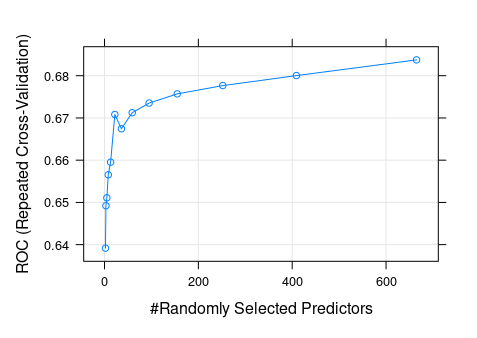
\includegraphics[width=6.62in]{pictures/ROC_cross_validation} 

}

\caption{ Courbe ROC avec validation croisée}\label{fig:ROC}
\end{figure}

Le modèle ayant la meilleure prédiction par validation croisée est alors
le modèle final en sortie. On regardera ensuite les performances de
l'arbre apris sur le jeu test

\begin{Shaded}
\begin{Highlighting}[]
\NormalTok{decision }\OtherTok{\textless{}{-}}\NormalTok{ rfFit}\SpecialCharTok{$}\NormalTok{finalModel}

\CommentTok{\#  Prédiction du modèle}
\NormalTok{prediction }\OtherTok{\textless{}{-}} \FunctionTok{predict}\NormalTok{(decision,cancerTest)}
\CommentTok{\# la matrice de confusion}
\NormalTok{confMat }\OtherTok{\textless{}{-}} \FunctionTok{confusionMatrix}\NormalTok{(prediction,cancerTest}\SpecialCharTok{$}\NormalTok{Y)}
\FunctionTok{save}\NormalTok{(confMat, }\AttributeTok{file =} \StringTok{"data/confMat.RData"}\NormalTok{)}
\end{Highlighting}
\end{Shaded}

\begin{verbatim}
## $positive
## [1] "no"
## 
## $table
##           Reference
## Prediction  no yes
##        no  295 141
##        yes  12  11
## 
## $overall
##       Accuracy          Kappa  AccuracyLower  AccuracyUpper   AccuracyNull 
##   6.666667e-01   4.235474e-02   6.214823e-01   7.096866e-01   6.688453e-01 
## AccuracyPValue  McnemarPValue 
##   5.612743e-01   4.264868e-25 
## 
## $byClass
##          Sensitivity          Specificity       Pos Pred Value 
##           0.96091205           0.07236842           0.67660550 
##       Neg Pred Value            Precision               Recall 
##           0.47826087           0.67660550           0.96091205 
##                   F1           Prevalence       Detection Rate 
##           0.79407806           0.66884532           0.64270153 
## Detection Prevalence    Balanced Accuracy 
##           0.94989107           0.51664024 
## 
## $mode
## [1] "sens_spec"
## 
## $dots
## list()
## 
## attr(,"class")
## [1] "confusionMatrix"
\end{verbatim}

l'Accuracy indique la proportion de bien classé (le pourcentage de
nombres d'individus bien classés sur le jeu text). Il indique 67\%. la
sensitivité qui indique la proportion de vraies décédées du cancer est
de 96\%. On a 7\% qui sont survécues ou qont mortes d'une autre façon
différente non causée par le cancer du sein.

\begin{enumerate}
\def\labelenumi{\arabic{enumi}.}
\setcounter{enumi}{1}
\item
  Méthode de prédiction SVM

  \begin{itemize}
  \tightlist
  \item
    Sur le jeu d'apprentissage créé précédemment, on apllique les deux
    méthodes de SVM: linéaire et à noyaux.
  \end{itemize}
\end{enumerate}

\begin{Shaded}
\begin{Highlighting}[]
\NormalTok{linearsvm }\OtherTok{\textless{}{-}}  \FunctionTok{svm}\NormalTok{(}\AttributeTok{formula =}\NormalTok{ Y}\SpecialCharTok{\textasciitilde{}}\NormalTok{., }
                  \AttributeTok{data =}\NormalTok{ cancerTraining,}
                  \AttributeTok{type =} \StringTok{\textquotesingle{}C{-}classification\textquotesingle{}}\NormalTok{, }
                  \AttributeTok{kernel =} \StringTok{\textquotesingle{}linear\textquotesingle{}}
\NormalTok{                  )}


\NormalTok{gaussiansvm }\OtherTok{\textless{}{-}} \FunctionTok{svm}\NormalTok{(}\AttributeTok{formula =}\NormalTok{ Y}\SpecialCharTok{\textasciitilde{}}\NormalTok{., }
                   \AttributeTok{data =}\NormalTok{ cancerTraining,}
                   \AttributeTok{type =} \StringTok{\textquotesingle{}C{-}classification\textquotesingle{}}\NormalTok{, }
                   \AttributeTok{kernel =} \StringTok{\textquotesingle{}radial\textquotesingle{}}
\NormalTok{                   )}
\end{Highlighting}
\end{Shaded}

\begin{itemize}
\tightlist
\item
  Prédiction sur le jeu test
\end{itemize}

\begin{Shaded}
\begin{Highlighting}[]
\NormalTok{linearpred   }\OtherTok{\textless{}{-}} \FunctionTok{predict}\NormalTok{(linearsvm, }\AttributeTok{newdata =}\NormalTok{ cancerTest)}
\NormalTok{gaussianpred }\OtherTok{\textless{}{-}} \FunctionTok{predict}\NormalTok{(gaussiansvm, }\AttributeTok{newdata =}\NormalTok{ cancerTest)}

\NormalTok{confMatSVM\_lin }\OtherTok{\textless{}{-}} \FunctionTok{confusionMatrix}\NormalTok{(}\AttributeTok{data=}\NormalTok{linearpred,cancerTest}\SpecialCharTok{$}\NormalTok{Y)}
\NormalTok{confMatSVM\_gau }\OtherTok{\textless{}{-}} \FunctionTok{confusionMatrix}\NormalTok{(}\AttributeTok{data=}\NormalTok{gaussianpred,cancerTest}\SpecialCharTok{$}\NormalTok{Y)}
\FunctionTok{save}\NormalTok{(confMatSVM\_lin,}\AttributeTok{file=}\StringTok{"data/confMatSVM\_lin.RData"}\NormalTok{)}
\FunctionTok{save}\NormalTok{(confMatSVM\_gau,}\AttributeTok{file=}\StringTok{"data/confMatSVM\_gau.RData"}\NormalTok{)}
\end{Highlighting}
\end{Shaded}

\begin{Shaded}
\begin{Highlighting}[]
\FunctionTok{load}\NormalTok{(}\AttributeTok{file=}\StringTok{"data/confMatSVM\_lin.RData"}\NormalTok{)}
\FunctionTok{load}\NormalTok{(}\AttributeTok{file=}\StringTok{"data/confMatSVM\_gau.RData"}\NormalTok{)}
\FunctionTok{print}\NormalTok{(confMatSVM\_lin)}
\end{Highlighting}
\end{Shaded}

\begin{verbatim}
## $positive
## [1] "no"
## 
## $table
##           Reference
## Prediction  no yes
##        no  213  89
##        yes  94  63
## 
## $overall
##       Accuracy          Kappa  AccuracyLower  AccuracyUpper   AccuracyNull 
##      0.6013072      0.1073930      0.5548900      0.6464103      0.6688453 
## AccuracyPValue  McnemarPValue 
##      0.9989714      0.7674680 
## 
## $byClass
##          Sensitivity          Specificity       Pos Pred Value 
##            0.6938111            0.4144737            0.7052980 
##       Neg Pred Value            Precision               Recall 
##            0.4012739            0.7052980            0.6938111 
##                   F1           Prevalence       Detection Rate 
##            0.6995074            0.6688453            0.4640523 
## Detection Prevalence    Balanced Accuracy 
##            0.6579521            0.5541424 
## 
## $mode
## [1] "sens_spec"
## 
## $dots
## list()
## 
## attr(,"class")
## [1] "confusionMatrix"
\end{verbatim}

\begin{Shaded}
\begin{Highlighting}[]
\FunctionTok{print}\NormalTok{(confMatSVM\_gau)}
\end{Highlighting}
\end{Shaded}

\begin{verbatim}
## $positive
## [1] "no"
## 
## $table
##           Reference
## Prediction  no yes
##        no  287 129
##        yes  20  23
## 
## $overall
##       Accuracy          Kappa  AccuracyLower  AccuracyUpper   AccuracyNull 
##   6.753813e-01   1.052163e-01   6.304286e-01   7.180558e-01   6.688453e-01 
## AccuracyPValue  McnemarPValue 
##   4.041379e-01   8.933764e-19 
## 
## $byClass
##          Sensitivity          Specificity       Pos Pred Value 
##            0.9348534            0.1513158            0.6899038 
##       Neg Pred Value            Precision               Recall 
##            0.5348837            0.6899038            0.9348534 
##                   F1           Prevalence       Detection Rate 
##            0.7939142            0.6688453            0.6252723 
## Detection Prevalence    Balanced Accuracy 
##            0.9063181            0.5430846 
## 
## $mode
## [1] "sens_spec"
## 
## $dots
## list()
## 
## attr(,"class")
## [1] "confusionMatrix"
\end{verbatim}

Au vu des deux matrices de confusion précédentes, la méthode SVM par
noyau gaussien est plus adaptée.

\begin{enumerate}
\def\labelenumi{\arabic{enumi}.}
\setcounter{enumi}{2}
\tightlist
\item
  Méthode de prédiction avec pénalité
\end{enumerate}

Nous disposons de trois méthodes pour la régression pénalisée: Lasso,
Ridge et Elastic-net. Soient le jeu d'apprentissage
\emph{cancerTraining} et le jeu test \emph{cancerTest} crées
précédemment.

\begin{Shaded}
\begin{Highlighting}[]
\CommentTok{\#jeu d\textquotesingle{}apprentissage }
\NormalTok{y.train }\OtherTok{\textless{}{-}}\NormalTok{ cancerTraining }\SpecialCharTok{\%\textgreater{}\%} 
  \FunctionTok{select}\NormalTok{(Y) }\SpecialCharTok{\%\textgreater{}\%}
  \FunctionTok{as.matrix}\NormalTok{()}
\NormalTok{y.test }\OtherTok{\textless{}{-}}\NormalTok{ cancerTest }\SpecialCharTok{\%\textgreater{}\%} 
  \FunctionTok{select}\NormalTok{(Y) }\SpecialCharTok{\%\textgreater{}\%} 
  \FunctionTok{as.matrix}\NormalTok{()}

\NormalTok{x.train }\OtherTok{\textless{}{-}}\NormalTok{ cancerTraining }\SpecialCharTok{\%\textgreater{}\%} 
  \FunctionTok{select}\NormalTok{(}\SpecialCharTok{{-}}\NormalTok{Y) }\SpecialCharTok{\%\textgreater{}\%} 
  \FunctionTok{as.matrix}\NormalTok{()}

\NormalTok{x.test }\OtherTok{\textless{}{-}}\NormalTok{ cancerTest }\SpecialCharTok{\%\textgreater{}\%} 
  \FunctionTok{select}\NormalTok{(}\SpecialCharTok{{-}}\NormalTok{Y) }\SpecialCharTok{\%\textgreater{}\%} 
  \FunctionTok{as.matrix}\NormalTok{()}
\end{Highlighting}
\end{Shaded}

\begin{itemize}
\tightlist
\item
  Pénalité Ridge
\end{itemize}

\begin{Shaded}
\begin{Highlighting}[]
\NormalTok{model.ridge }\OtherTok{\textless{}{-}} \FunctionTok{glmnet}\NormalTok{(x.train,y.train,}\AttributeTok{family =} \StringTok{"binomial"}\NormalTok{,}\AttributeTok{alpha=}\DecValTok{0}\NormalTok{)}
\FunctionTok{plot}\NormalTok{(model.ridge)}
\end{Highlighting}
\end{Shaded}

\begin{figure}

{\centering 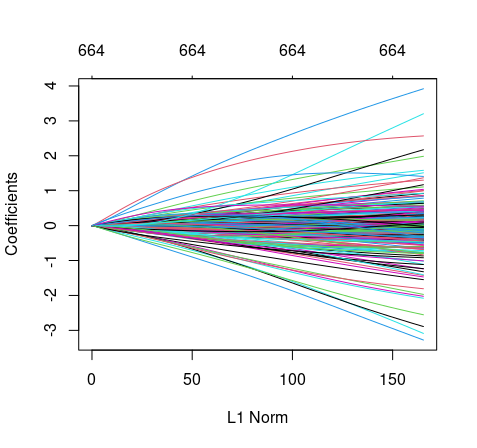
\includegraphics[width=0.5\linewidth]{pictures/ridge} 

}

\caption{ Modèle ridge}\label{fig:fig_ridge}
\end{figure}

\newpage

\begin{itemize}
\tightlist
\item
  Lasso
\end{itemize}

\begin{Shaded}
\begin{Highlighting}[]
\NormalTok{model.lasso }\OtherTok{\textless{}{-}} \FunctionTok{glmnet}\NormalTok{(x.train,y.train,}\AttributeTok{family =} \StringTok{"binomial"}\NormalTok{,}\AttributeTok{alpha=}\DecValTok{1}\NormalTok{)}
\end{Highlighting}
\end{Shaded}

\begin{figure}

{\centering 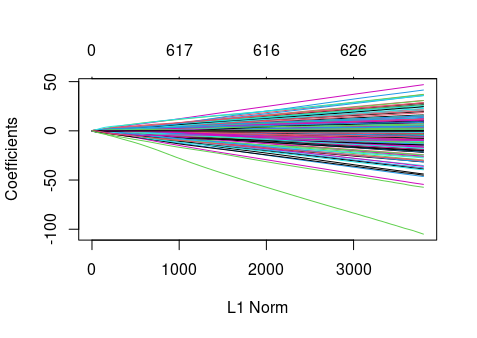
\includegraphics[width=0.5\linewidth]{pictures/lasso} 

}

\caption{ Modèle Lasso}\label{fig:fig_lasso}
\end{figure}

\begin{itemize}
\tightlist
\item
  Elastic net
\end{itemize}

\begin{Shaded}
\begin{Highlighting}[]
\NormalTok{model.elastic\_net }\OtherTok{\textless{}{-}} \FunctionTok{glmnet}\NormalTok{(x.train,y.train,}\AttributeTok{family =} \StringTok{"binomial"}\NormalTok{,}\AttributeTok{alpha=}\NormalTok{.}\DecValTok{5}\NormalTok{)}
\end{Highlighting}
\end{Shaded}

\begin{figure}

{\centering 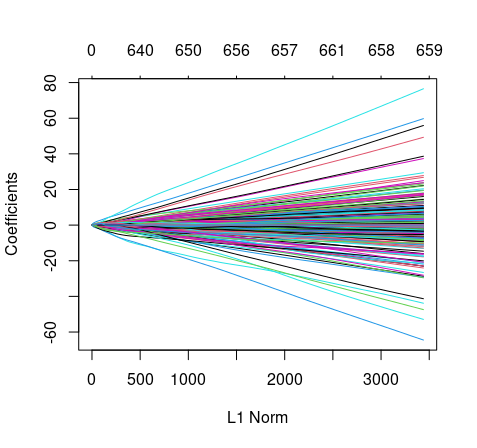
\includegraphics[width=0.5\linewidth]{pictures/elastic_net} 

}

\caption{ Modèle Elastic net}\label{fig:fig_EN}
\end{figure}

Nous choisirons la méthode \emph{elastic net} en procédant par
validation croisée. Car c'est un bon compromis entre les deux.

\begin{Shaded}
\begin{Highlighting}[]
\NormalTok{cancer.cv }\OtherTok{\textless{}{-}} \FunctionTok{cv.glmnet}\NormalTok{(x.train,y.train,}\AttributeTok{nfolds=}\DecValTok{20}\NormalTok{,}\AttributeTok{family=}\StringTok{"binomial"}\NormalTok{)}
\NormalTok{cancer.cv}\SpecialCharTok{$}\NormalTok{lambda.min}
\NormalTok{model.EN.cv }\OtherTok{\textless{}{-}} \FunctionTok{glmnet}\NormalTok{(x.train,y.train,}\AttributeTok{family=}\StringTok{"binomial"}\NormalTok{,}\AttributeTok{alpha=}\FloatTok{0.5}\NormalTok{,}\AttributeTok{nlambda=}\DecValTok{1}\NormalTok{,}\AttributeTok{lambda=}\NormalTok{cancer.cv}\SpecialCharTok{$}\NormalTok{lambda.min)}
\end{Highlighting}
\end{Shaded}

\newpage

\begin{itemize}
\tightlist
\item
  Prédiction du modèle sur le jeu test
\end{itemize}

\begin{Shaded}
\begin{Highlighting}[]
\NormalTok{cancerpredict.EN.cv }\OtherTok{\textless{}{-}} \FunctionTok{predict}\NormalTok{(model.EN.cv,x.train,}
                               \AttributeTok{type=}\StringTok{"response"}\NormalTok{,}
                               \AttributeTok{family=}\StringTok{"binomial"}
\NormalTok{                               )}
\NormalTok{results }\OtherTok{\textless{}{-}} \FunctionTok{tibble}\NormalTok{(}\AttributeTok{proba=}\NormalTok{cancerpredict.EN.cv,}
                  \AttributeTok{y.pred=}\FunctionTok{round}\NormalTok{(cancerpredict.EN.cv),}
                  \AttributeTok{y.truth=}\NormalTok{(y.train}\SpecialCharTok{==}\StringTok{"yes"}\NormalTok{)}\SpecialCharTok{*}\DecValTok{1}
\NormalTok{                  )}
\NormalTok{results}
\NormalTok{cfMat.EN }\OtherTok{\textless{}{-}} \FunctionTok{confusionMatrix}\NormalTok{(}\AttributeTok{data =} \FunctionTok{as\_factor}\NormalTok{(results}\SpecialCharTok{$}\NormalTok{y.pred),}
                            \FunctionTok{as\_factor}\NormalTok{(results}\SpecialCharTok{$}\NormalTok{y.truth)}
\NormalTok{                            )}
\FunctionTok{save}\NormalTok{(cfMat.EN,}\AttributeTok{file =} \StringTok{"pictures/cfMat\_acp.RData"}\NormalTok{)}
\end{Highlighting}
\end{Shaded}

\begin{verbatim}
## $positive
## [1] "0"
## 
## $table
##           Reference
## Prediction   0   1
##          0 860 240
##          1  64 216
## 
## $overall
##       Accuracy          Kappa  AccuracyLower  AccuracyUpper   AccuracyNull 
##   7.797101e-01   4.482323e-01   7.568981e-01   8.013246e-01   6.695652e-01 
## AccuracyPValue  McnemarPValue 
##   1.391578e-19   1.048789e-23 
## 
## $byClass
##          Sensitivity          Specificity       Pos Pred Value 
##            0.9307359            0.4736842            0.7818182 
##       Neg Pred Value            Precision               Recall 
##            0.7714286            0.7818182            0.9307359 
##                   F1           Prevalence       Detection Rate 
##            0.8498024            0.6695652            0.6231884 
## Detection Prevalence    Balanced Accuracy 
##            0.7971014            0.7022101 
## 
## $mode
## [1] "sens_spec"
## 
## $dots
## list()
## 
## attr(,"class")
## [1] "confusionMatrix"
\end{verbatim}

La matrice de confusion donne un bon taux de classement (78\%) sur le
jeu test avec une bonne sensitivité de 93\% et une spécificité assez
faible de 47.4\%.

\begin{enumerate}
\def\labelenumi{\alph{enumi}.}
\setcounter{enumi}{1}
\tightlist
\item
  par ACP
\end{enumerate}

\begin{itemize}
\tightlist
\item
  Réduction de dimension par ACP
\end{itemize}

Nous choisissons de prendre les variables nécessaires qui expliquent
70\% du résultat de l'ACP

\begin{Shaded}
\begin{Highlighting}[]
\NormalTok{acp }\OtherTok{\textless{}{-}}\NormalTok{ datacancer }\SpecialCharTok{\%\textgreater{}\%} 
  \FunctionTok{select}\NormalTok{(}\SpecialCharTok{{-}}\NormalTok{Y) }\SpecialCharTok{\%\textgreater{}\%} \FunctionTok{as.matrix}\NormalTok{() }\SpecialCharTok{\%\textgreater{}\%} 
  \FunctionTok{prcomp}\NormalTok{()}

\CommentTok{\# selection des variables avec 70\% }
\NormalTok{nvar }\OtherTok{\textless{}{-}} \FunctionTok{which}\NormalTok{(}\FunctionTok{cumsum}\NormalTok{(acp[[}\StringTok{"sdev"}\NormalTok{]])}\SpecialCharTok{/}\FunctionTok{sum}\NormalTok{(acp[[}\StringTok{"sdev"}\NormalTok{]])}\SpecialCharTok{\textgreater{}}\NormalTok{.}\DecValTok{7}\NormalTok{)}

\NormalTok{cancerTraining\_ACP }\OtherTok{\textless{}{-}} \FunctionTok{as\_tibble}\NormalTok{(acp}\SpecialCharTok{$}\NormalTok{x[,}\DecValTok{1}\SpecialCharTok{:}\NormalTok{nvar]) }\SpecialCharTok{\%\textgreater{}\%} 
                   \FunctionTok{mutate}\NormalTok{(}\AttributeTok{Y=}\NormalTok{datacancer}\SpecialCharTok{$}\NormalTok{Y,}
                   \AttributeTok{.before=}\StringTok{"PC1"}
\NormalTok{                     ) }\SpecialCharTok{\%\textgreater{}\%} 
                   \FunctionTok{slice}\NormalTok{(}\AttributeTok{n=}\NormalTok{inTrain)}

\NormalTok{cancerTest\_ACP }\OtherTok{\textless{}{-}} \FunctionTok{as\_tibble}\NormalTok{(acp}\SpecialCharTok{$}\NormalTok{x[,}\DecValTok{1}\SpecialCharTok{:}\NormalTok{nvar]) }\SpecialCharTok{\%\textgreater{}\%} 
                   \FunctionTok{mutate}\NormalTok{(}\AttributeTok{Y=}\NormalTok{datacancer}\SpecialCharTok{$}\NormalTok{Y,}
                   \AttributeTok{.before=}\StringTok{"PC1"}
\NormalTok{                     ) }\SpecialCharTok{\%\textgreater{}\%} 
                   \FunctionTok{slice}\NormalTok{(}\AttributeTok{n=}\SpecialCharTok{{-}}\NormalTok{inTrain)}
\end{Highlighting}
\end{Shaded}

On a une diminution de nombre de variable de 244.

\begin{enumerate}
\def\labelenumi{\arabic{enumi}.}
\tightlist
\item
  Méthodes de prédiction avec forêt aléatoire
\end{enumerate}

\begin{Shaded}
\begin{Highlighting}[]
\NormalTok{rfFit\_ACP }\OtherTok{\textless{}{-}} \FunctionTok{train}\NormalTok{(}
\NormalTok{  Y }\SpecialCharTok{\textasciitilde{}}\NormalTok{ .,}
  \AttributeTok{data =}\NormalTok{ cancerTraining\_ACP,}
  \AttributeTok{method =} \StringTok{"rf"}\NormalTok{,}
  \AttributeTok{tuneLength =} \DecValTok{13}\NormalTok{, }\CommentTok{\#donne le nombre de valeurs à essayer pour chaque paramètre à faire varier (ici nombre de variables à prendre en compte)}
  \AttributeTok{trControl =}\NormalTok{ ctrl,}
  \AttributeTok{metric =} \StringTok{"ROC"}
\NormalTok{)}
\FunctionTok{plot}\NormalTok{(rfit)}
\end{Highlighting}
\end{Shaded}

\begin{figure}

{\centering 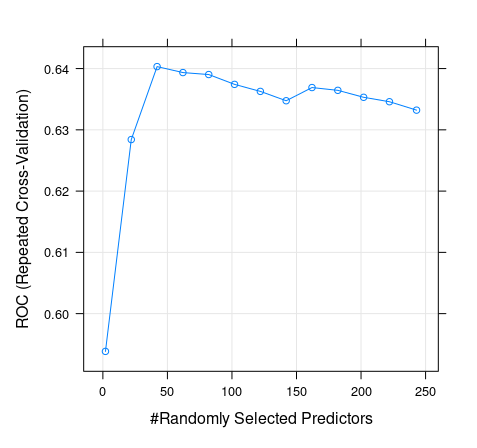
\includegraphics[width=0.5\linewidth]{pictures/ROC_cross_validation_acp} 

}

\caption{Courbe ROC par validation croisée/Avec réduction de dimension}\label{fig:roc_acp}
\end{figure}

\begin{verbatim}
## $positive
## [1] "no"
## 
## $table
##           Reference
## Prediction  no yes
##        no  297 146
##        yes  10   6
## 
## $overall
##       Accuracy          Kappa  AccuracyLower  AccuracyUpper   AccuracyNull 
##   6.601307e-01   8.913742e-03   6.147833e-01   7.033988e-01   6.688453e-01 
## AccuracyPValue  McnemarPValue 
##   6.738991e-01   3.132446e-27 
## 
## $byClass
##          Sensitivity          Specificity       Pos Pred Value 
##           0.96742671           0.03947368           0.67042889 
##       Neg Pred Value            Precision               Recall 
##           0.37500000           0.67042889           0.96742671 
##                   F1           Prevalence       Detection Rate 
##           0.79200000           0.66884532           0.64705882 
## Detection Prevalence    Balanced Accuracy 
##           0.96514161           0.50345020 
## 
## $mode
## [1] "sens_spec"
## 
## $dots
## list()
## 
## attr(,"class")
## [1] "confusionMatrix"
\end{verbatim}

66\% des individus sont bien classés selon cette méthode avec un bon
taux du nombre de patientes décédées (97\%). Cependant la spécifité est
très faible (4\%)

\begin{enumerate}
\def\labelenumi{\arabic{enumi}.}
\setcounter{enumi}{1}
\tightlist
\item
  Méthode de prédiction SVM
\end{enumerate}

\begin{itemize}
\tightlist
\item
  On réutilise les jeux d'apprentissage et de test précédemment dans
  cette dsection ( \emph{cancderTraining\_ACP} et
  \emph{canccerTest\_ACP} ).
\end{itemize}

\begin{Shaded}
\begin{Highlighting}[]
\NormalTok{linearsvm\_acp }\OtherTok{\textless{}{-}}  \FunctionTok{svm}\NormalTok{(}\AttributeTok{formula =}\NormalTok{ Y}\SpecialCharTok{\textasciitilde{}}\NormalTok{., }
                  \AttributeTok{data =}\NormalTok{ cancerTraining\_ACP,}
                  \AttributeTok{type =} \StringTok{\textquotesingle{}C{-}classification\textquotesingle{}}\NormalTok{, }
                  \AttributeTok{kernel =} \StringTok{\textquotesingle{}linear\textquotesingle{}}\NormalTok{)}

\NormalTok{gaussiansvm\_acp }\OtherTok{\textless{}{-}} \FunctionTok{svm}\NormalTok{(}\AttributeTok{formula =}\NormalTok{ Y}\SpecialCharTok{\textasciitilde{}}\NormalTok{., }
                   \AttributeTok{data =}\NormalTok{ cancerTraining\_ACP,}
                   \AttributeTok{type =} \StringTok{\textquotesingle{}C{-}classification\textquotesingle{}}\NormalTok{, }
                   \AttributeTok{kernel =} \StringTok{\textquotesingle{}radial\textquotesingle{}}\NormalTok{)}
\end{Highlighting}
\end{Shaded}

\begin{itemize}
\tightlist
\item
  Prédiction sur le jeu test et matrice de confusion
\end{itemize}

\begin{Shaded}
\begin{Highlighting}[]
\NormalTok{linearpred\_acp      }\OtherTok{\textless{}{-}} \FunctionTok{predict}\NormalTok{(linearsvm\_acp, }\AttributeTok{newdata =}\NormalTok{ cancerTest\_ACP)}
\NormalTok{gaussianpred\_acp    }\OtherTok{\textless{}{-}} \FunctionTok{predict}\NormalTok{(gaussiansvm\_acp, }\AttributeTok{newdata =}\NormalTok{ cancerTest\_ACP)}
\NormalTok{confMat\_svm\_acp\_lin }\OtherTok{\textless{}{-}} \FunctionTok{confusionMatrix}\NormalTok{(}\AttributeTok{data=}\NormalTok{linearpred\_acp,cancerTest\_ACP}\SpecialCharTok{$}\NormalTok{Y)}
\NormalTok{confMat\_svm\_acp\_gau }\OtherTok{\textless{}{-}} \FunctionTok{confusionMatrix}\NormalTok{(}\AttributeTok{data=}\NormalTok{gaussianpred\_acp,cancerTest\_ACP}\SpecialCharTok{$}\NormalTok{Y)}

\FunctionTok{save}\NormalTok{(confMat\_svm\_acp\_lin, }\AttributeTok{file =} \StringTok{"data/confMat\_svm\_acp\_lin.RData"}\NormalTok{)}
\FunctionTok{save}\NormalTok{(confMat\_svm\_acp\_gau,}\AttributeTok{file =} \StringTok{"data/confMat\_svm\_acp\_gau.RData"}\NormalTok{)}
\end{Highlighting}
\end{Shaded}

\begin{Shaded}
\begin{Highlighting}[]
\FunctionTok{load}\NormalTok{(}\StringTok{"data/confMat\_svm\_acp\_lin.RData"}\NormalTok{)}
\FunctionTok{load}\NormalTok{(}\StringTok{"data/confMat\_svm\_acp\_gau.RData"}\NormalTok{)}

\NormalTok{confMat\_svm\_acp\_lin}
\end{Highlighting}
\end{Shaded}

\begin{verbatim}
## $positive
## [1] "no"
## 
## $table
##           Reference
## Prediction  no yes
##        no  240 110
##        yes  67  42
## 
## $overall
##       Accuracy          Kappa  AccuracyLower  AccuracyUpper   AccuracyNull 
##    0.614379085    0.062541108    0.568139669    0.659134549    0.668845316 
## AccuracyPValue  McnemarPValue 
##    0.993830902    0.001594487 
## 
## $byClass
##          Sensitivity          Specificity       Pos Pred Value 
##            0.7817590            0.2763158            0.6857143 
##       Neg Pred Value            Precision               Recall 
##            0.3853211            0.6857143            0.7817590 
##                   F1           Prevalence       Detection Rate 
##            0.7305936            0.6688453            0.5228758 
## Detection Prevalence    Balanced Accuracy 
##            0.7625272            0.5290374 
## 
## $mode
## [1] "sens_spec"
## 
## $dots
## list()
## 
## attr(,"class")
## [1] "confusionMatrix"
\end{verbatim}

\begin{Shaded}
\begin{Highlighting}[]
\NormalTok{confMat\_svm\_acp\_gau}
\end{Highlighting}
\end{Shaded}

\begin{verbatim}
## $positive
## [1] "no"
## 
## $table
##           Reference
## Prediction  no yes
##        no  305 145
##        yes   2   7
## 
## $overall
##       Accuracy          Kappa  AccuracyLower  AccuracyUpper   AccuracyNull 
##   6.797386e-01   5.185279e-02   6.349081e-01   7.222341e-01   6.688453e-01 
## AccuracyPValue  McnemarPValue 
##   3.293343e-01   1.106874e-31 
## 
## $byClass
##          Sensitivity          Specificity       Pos Pred Value 
##           0.99348534           0.04605263           0.67777778 
##       Neg Pred Value            Precision               Recall 
##           0.77777778           0.67777778           0.99348534 
##                   F1           Prevalence       Detection Rate 
##           0.80581242           0.66884532           0.66448802 
## Detection Prevalence    Balanced Accuracy 
##           0.98039216           0.51976899 
## 
## $mode
## [1] "sens_spec"
## 
## $dots
## list()
## 
## attr(,"class")
## [1] "confusionMatrix"
\end{verbatim}

\begin{enumerate}
\def\labelenumi{\arabic{enumi}.}
\setcounter{enumi}{2}
\tightlist
\item
  Méthode de prédiction avec pénalité
\end{enumerate}

\begin{Shaded}
\begin{Highlighting}[]
\CommentTok{\#jeu d\textquotesingle{}apprentissage }
\NormalTok{y.train\_acp }\OtherTok{\textless{}{-}}\NormalTok{ cancerTraining\_ACP }\SpecialCharTok{\%\textgreater{}\%} 
  \FunctionTok{select}\NormalTok{(Y) }\SpecialCharTok{\%\textgreater{}\%}
  \FunctionTok{as.matrix}\NormalTok{()}

\NormalTok{x.train\_acp }\OtherTok{\textless{}{-}}\NormalTok{ cancerTraining\_ACP }\SpecialCharTok{\%\textgreater{}\%} 
  \FunctionTok{select}\NormalTok{(}\SpecialCharTok{{-}}\NormalTok{Y) }\SpecialCharTok{\%\textgreater{}\%} 
  \FunctionTok{as.matrix}\NormalTok{()}
\end{Highlighting}
\end{Shaded}

\begin{itemize}
\tightlist
\item
  Pénalité Ridge
\end{itemize}

\begin{Shaded}
\begin{Highlighting}[]
\NormalTok{model.ridge\_acp }\OtherTok{\textless{}{-}} \FunctionTok{glmnet}\NormalTok{(x.train\_acp,y.train\_acp,}\AttributeTok{family =} \StringTok{"binomial"}\NormalTok{ ,}\AttributeTok{alpha=}\DecValTok{0}\NormalTok{)}
\FunctionTok{plot}\NormalTok{(model.ridge\_acp)}
\end{Highlighting}
\end{Shaded}

\begin{figure}

{\centering 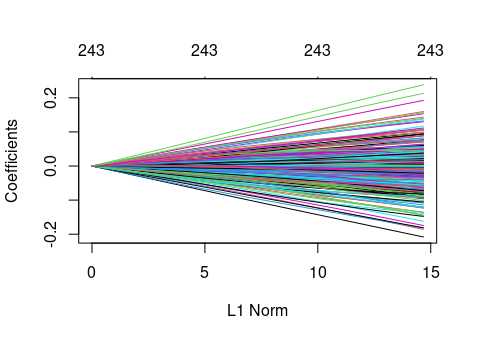
\includegraphics[width=0.5\linewidth]{pictures/ridge_acp} 

}

\caption{Méthde de Ridge}\label{fig:ridge_acp}
\end{figure}

\begin{itemize}
\tightlist
\item
  Pénalité Lasso
\end{itemize}

\begin{Shaded}
\begin{Highlighting}[]
\NormalTok{model.lasso\_acp }\OtherTok{\textless{}{-}} \FunctionTok{glmnet}\NormalTok{(x.train\_acp,y.train\_acp,}\AttributeTok{family =} \StringTok{"binomial"}\NormalTok{ , }\AttributeTok{alpha=}\DecValTok{1}\NormalTok{)}
\FunctionTok{plot}\NormalTok{(model.lasso\_acp)}
\end{Highlighting}
\end{Shaded}

\begin{figure}

{\centering 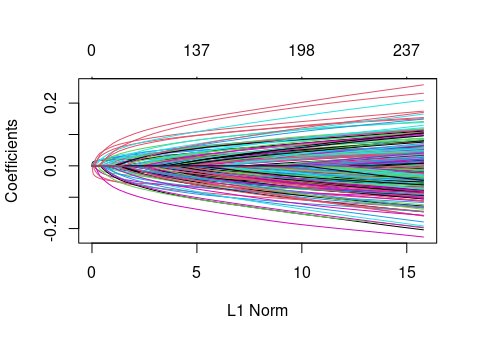
\includegraphics[width=0.5\linewidth]{pictures/lasso_acp} 

}

\caption{Pénalité Lasso}\label{fig:lasso_acp}
\end{figure}

\begin{itemize}
\tightlist
\item
  Pénalité Elastic net
\end{itemize}

\begin{Shaded}
\begin{Highlighting}[]
\NormalTok{model.elastic\_net\_acp }\OtherTok{\textless{}{-}} \FunctionTok{glmnet}\NormalTok{(x.train\_acp,y.train\_acp,}\AttributeTok{family =} \StringTok{"binomial"}\NormalTok{ , }\AttributeTok{alpha=}\NormalTok{.}\DecValTok{5}\NormalTok{)}
\FunctionTok{plot}\NormalTok{(model.elastic\_net\_acp)}
\end{Highlighting}
\end{Shaded}

\begin{figure}

{\centering 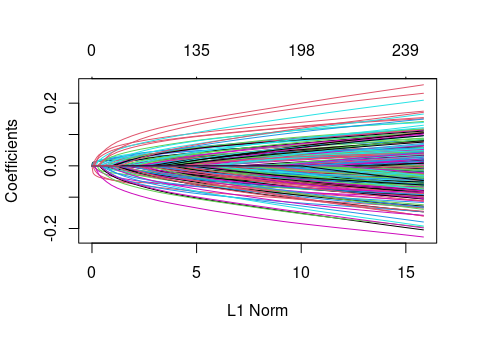
\includegraphics[width=0.5\linewidth]{pictures/elastic_net_acp} 

}

\caption{Elastic net}\label{fig:elastic_net_acp}
\end{figure}

\begin{itemize}
\tightlist
\item
  Prédition avec elastic net
\end{itemize}

\begin{Shaded}
\begin{Highlighting}[]
\NormalTok{cancer.cv\_acp }\OtherTok{\textless{}{-}} \FunctionTok{cv.glmnet}\NormalTok{(x.train\_acp,y.train\_acp,}
                           \AttributeTok{nfolds=}\DecValTok{10}\NormalTok{,}
                           \AttributeTok{family=}\StringTok{"binomial"} 
\NormalTok{                           )}
\NormalTok{cancer.cv\_acp}\SpecialCharTok{$}\NormalTok{lambda.min}
\NormalTok{model.EN.cv\_acp }\OtherTok{\textless{}{-}} \FunctionTok{glmnet}\NormalTok{(x.train\_acp,}
\NormalTok{                          y.train\_acp,}
                          \AttributeTok{family=}\StringTok{"binomial"}\NormalTok{ ,}
                          \AttributeTok{alpha=}\FloatTok{0.5}\NormalTok{,}\AttributeTok{nlambda=}\DecValTok{100}\NormalTok{,}
                          \AttributeTok{lambda=}\NormalTok{cancer.cv\_acp}\SpecialCharTok{$}\NormalTok{lambda.min}
\NormalTok{                          )}

\NormalTok{cancerpredict.EN.cv\_acp }\OtherTok{\textless{}{-}} \FunctionTok{predict}\NormalTok{(model.EN.cv\_acp,x.train\_acp,}
                                   \AttributeTok{type=}\StringTok{"response"}\NormalTok{, }\AttributeTok{family=}\StringTok{"binomial"} 
\NormalTok{                                   )}
\NormalTok{results\_acp }\OtherTok{\textless{}{-}} \FunctionTok{tibble}\NormalTok{(}\AttributeTok{proba=}\NormalTok{cancerpredict.EN.cv\_acp,}
                      \AttributeTok{pred=}\FunctionTok{round}\NormalTok{(cancerpredict.EN.cv\_acp),}
                      \AttributeTok{y.truth=}\NormalTok{(y.train\_acp}\SpecialCharTok{==}\StringTok{"yes"}\NormalTok{) }\SpecialCharTok{*}\DecValTok{1} 
\NormalTok{                      )}
\NormalTok{results\_acp}
\NormalTok{confMat\_EN\_acp }\OtherTok{\textless{}{-}} \FunctionTok{confusionMatrix}\NormalTok{(}\AttributeTok{data=}\FunctionTok{as\_factor}\NormalTok{(results\_acp}\SpecialCharTok{$}\NormalTok{pred),}
                                  \FunctionTok{as\_factor}\NormalTok{(results\_acp}\SpecialCharTok{$}\NormalTok{y.truth)}
\NormalTok{                                  )}
\FunctionTok{save}\NormalTok{(confMat\_EN\_acp,}\AttributeTok{file =} \StringTok{"data/confMat\_EN\_acp.RData"}\NormalTok{)}
\end{Highlighting}
\end{Shaded}

\begin{itemize}
\tightlist
\item
  Matrice de confusion
\end{itemize}

\begin{verbatim}
## $positive
## [1] "0"
## 
## $table
##           Reference
## Prediction   0   1
##          0 876 313
##          1  48 143
## 
## $overall
##       Accuracy          Kappa  AccuracyLower  AccuracyUpper   AccuracyNull 
##   7.384058e-01   3.068009e-01   7.143632e-01   7.614288e-01   6.695652e-01 
## AccuracyPValue  McnemarPValue 
##   1.750297e-08   6.817361e-44 
## 
## $byClass
##          Sensitivity          Specificity       Pos Pred Value 
##            0.9480519            0.3135965            0.7367536 
##       Neg Pred Value            Precision               Recall 
##            0.7486911            0.7367536            0.9480519 
##                   F1           Prevalence       Detection Rate 
##            0.8291529            0.6695652            0.6347826 
## Detection Prevalence    Balanced Accuracy 
##            0.8615942            0.6308242 
## 
## $mode
## [1] "sens_spec"
## 
## $dots
## list()
## 
## attr(,"class")
## [1] "confusionMatrix"
\end{verbatim}

On a 74\% d'individus bien classés mais avec un mauvais taux de vrai
négatif (seulement 31,4\% des individus non décédées du cancer sont
détectés). Par contre on a une sensitivité de 95\%.

\newpage

\begin{enumerate}
\def\labelenumi{\alph{enumi}.}
\setcounter{enumi}{2}
\tightlist
\item
  par auto-encodeur
\end{enumerate}

Nous utiliserons le package \emph{keras} pour cette partie auto-encodeur
et considérons le jeu d'apprentissage \emph{cancerTraining}

\begin{itemize}
\tightlist
\item
  Préparation des données
\end{itemize}

\begin{Shaded}
\begin{Highlighting}[]
\NormalTok{y }\OtherTok{\textless{}{-}}\NormalTok{  cancerTraining }\SpecialCharTok{\%\textgreater{}\%} 
  \FunctionTok{mutate}\NormalTok{(}\AttributeTok{Y=}\FunctionTok{if\_else}\NormalTok{(Y}\SpecialCharTok{==}\StringTok{"no"}\NormalTok{,}\DecValTok{0}\NormalTok{,}\DecValTok{1}\NormalTok{)) }\SpecialCharTok{\%\textgreater{}\%} 
  \FunctionTok{select}\NormalTok{(Y)  }\SpecialCharTok{\%\textgreater{}\%} 
  \FunctionTok{as.matrix}\NormalTok{()}
\NormalTok{y }\OtherTok{\textless{}{-}} \FunctionTok{to\_categorical}\NormalTok{(y)}

\NormalTok{y.test }\OtherTok{\textless{}{-}}\NormalTok{  cancerTest }\SpecialCharTok{\%\textgreater{}\%} 
  \FunctionTok{mutate}\NormalTok{(}\AttributeTok{Y=}\FunctionTok{if\_else}\NormalTok{(Y}\SpecialCharTok{==}\StringTok{"no"}\NormalTok{,}\DecValTok{0}\NormalTok{,}\DecValTok{1}\NormalTok{)) }\SpecialCharTok{\%\textgreater{}\%} 
  \FunctionTok{select}\NormalTok{(Y) }\SpecialCharTok{\%\textgreater{}\%} 
  \FunctionTok{as.matrix}\NormalTok{()}
\NormalTok{y.test }\OtherTok{\textless{}{-}} \FunctionTok{to\_categorical}\NormalTok{(y.test)}


\NormalTok{x }\OtherTok{\textless{}{-}}\NormalTok{ cancerTraining }\SpecialCharTok{\%\textgreater{}\%} 
  \FunctionTok{select}\NormalTok{(}\SpecialCharTok{{-}}\NormalTok{Y) }\SpecialCharTok{\%\textgreater{}\%} 
  \FunctionTok{as.matrix}\NormalTok{()}
\NormalTok{x }\OtherTok{\textless{}{-}} \FunctionTok{array\_reshape}\NormalTok{(x,}\FunctionTok{dim}\NormalTok{(x))}

\NormalTok{x.test }\OtherTok{\textless{}{-}}\NormalTok{ cancerTest }\SpecialCharTok{\%\textgreater{}\%} 
  \FunctionTok{select}\NormalTok{(}\SpecialCharTok{{-}}\NormalTok{Y) }\SpecialCharTok{\%\textgreater{}\%} 
  \FunctionTok{as.matrix}\NormalTok{()}
\NormalTok{x.test }\OtherTok{\textless{}{-}} \FunctionTok{array\_reshape}\NormalTok{(x.test,}\FunctionTok{dim}\NormalTok{(x.test))}
\end{Highlighting}
\end{Shaded}

\begin{itemize}
\tightlist
\item
  Apprentissage
\end{itemize}

\begin{Shaded}
\begin{Highlighting}[]
\NormalTok{model }\OtherTok{\textless{}{-}} \FunctionTok{keras\_model\_sequential}\NormalTok{( }\AttributeTok{input\_shape =} \FunctionTok{c}\NormalTok{(}\DecValTok{665}\NormalTok{))}
\NormalTok{model }\SpecialCharTok{\%\textgreater{}\%} 
  \FunctionTok{layer\_dense}\NormalTok{(}\AttributeTok{units =} \DecValTok{64}\NormalTok{, }\AttributeTok{activation =} \StringTok{"relu"}\NormalTok{) }\SpecialCharTok{\%\textgreater{}\%} 
  \FunctionTok{layer\_dense}\NormalTok{(}\AttributeTok{units =} \DecValTok{32}\NormalTok{, }\AttributeTok{activation =} \StringTok{"sigmoid"}\NormalTok{) }\SpecialCharTok{\%\textgreater{}\%} 
  \FunctionTok{layer\_dense}\NormalTok{(}\AttributeTok{units =} \DecValTok{2}\NormalTok{, }\AttributeTok{activation =} \StringTok{"softmax"}\NormalTok{)  }

\NormalTok{model}

\NormalTok{model}\SpecialCharTok{$}\NormalTok{weights}



\CommentTok{\# compile}
\NormalTok{model }\SpecialCharTok{\%\textgreater{}\%} \FunctionTok{compile}\NormalTok{(}
\CommentTok{\#loss = \textquotesingle{}binary\_crossentropy\textquotesingle{},}
\AttributeTok{loss =} \FunctionTok{c}\NormalTok{(}\StringTok{"mean\_squared\_error"}\NormalTok{,}\StringTok{"binary\_crossentropy"}\NormalTok{),}
\AttributeTok{optimizer =} \StringTok{\textquotesingle{}adam\textquotesingle{}}\NormalTok{,}
\AttributeTok{metrics =} \FunctionTok{c}\NormalTok{(}\StringTok{\textquotesingle{}accuracy\textquotesingle{}}\NormalTok{)}
\NormalTok{)}

\CommentTok{\# Validation}

\CommentTok{\# Nous utilisons l\textquotesingle{}argument validation\_data pour apprendre sur le jeu de données test en faisant sortir}
\CommentTok{\# les erreurs quadratiques ansi que la proportion d\textquotesingle{}individus classée}
\NormalTok{history }\OtherTok{\textless{}{-}}\NormalTok{ model }\SpecialCharTok{\%\textgreater{}\%} \FunctionTok{fit}\NormalTok{(}
\NormalTok{x, y, }
\AttributeTok{epoch=}\DecValTok{100}\NormalTok{,}
\AttributeTok{batch\_size =} \DecValTok{128}\NormalTok{,}
\AttributeTok{validation\_data=}\FunctionTok{list}\NormalTok{(x.test,y.test)}
\CommentTok{\#validation\_split = 0.2,}
\CommentTok{\#verbose=FALSE}
\NormalTok{)}

\FunctionTok{str}\NormalTok{(history}\SpecialCharTok{$}\NormalTok{metrics)}
\FunctionTok{str}\NormalTok{(history}\SpecialCharTok{$}\NormalTok{params)}

\NormalTok{history}\SpecialCharTok{$}\NormalTok{metrics}\SpecialCharTok{$}\NormalTok{val\_accuracy[}\DecValTok{100}\NormalTok{]}
\NormalTok{history}\SpecialCharTok{$}\NormalTok{metrics}\SpecialCharTok{$}\NormalTok{val\_loss[}\DecValTok{100}\NormalTok{]}

\FunctionTok{plot}\NormalTok{(history)}
\end{Highlighting}
\end{Shaded}

\begin{figure}

{\centering 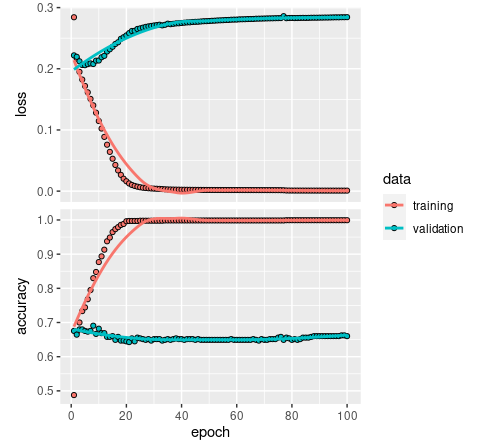
\includegraphics[width=1\linewidth]{pictures/keras} 

}

\caption{ Erreur moyenne quadratique et prédiction}\label{fig:keras}
\end{figure}

Avec keras, on a une précision de 61\% sur 100 itération et une erreur
quadratique moyenne de \(.302\).

\begin{itemize}
\tightlist
\item
  Prédicton
\end{itemize}

\begin{Shaded}
\begin{Highlighting}[]
\NormalTok{y.pred  }\OtherTok{\textless{}{-}}\NormalTok{ model }\SpecialCharTok{\%\textgreater{}\%}
  \FunctionTok{predict}\NormalTok{(x.test, }\AttributeTok{type =} \StringTok{"response"}\NormalTok{) }\SpecialCharTok{\%\textgreater{}\%} 
  \FunctionTok{apply}\NormalTok{(}\DecValTok{1}\NormalTok{,which.max)}\SpecialCharTok{{-}}\DecValTok{1}

\NormalTok{y.test\_test }\OtherTok{\textless{}{-}}\NormalTok{ y.test }\SpecialCharTok{\%\textgreater{}\%} 
    \FunctionTok{apply}\NormalTok{(}\DecValTok{1}\NormalTok{,which.max)}\SpecialCharTok{{-}}\DecValTok{1}


\FunctionTok{head}\NormalTok{(predictions, }\DecValTok{10}\NormalTok{)}


\NormalTok{datapred }\OtherTok{\textless{}{-}} \FunctionTok{data.frame}\NormalTok{(}\AttributeTok{x1=}\NormalTok{predictions[,}\DecValTok{1}\NormalTok{],}\AttributeTok{x2=}\NormalTok{predictions[,}\DecValTok{2}\NormalTok{],}\AttributeTok{y=}\NormalTok{y.pred)}

\FunctionTok{confusionMatrix}\NormalTok{(}\FunctionTok{as\_factor}\NormalTok{(y.pred), }\FunctionTok{as\_factor}\NormalTok{(y.test\_test))}
\end{Highlighting}
\end{Shaded}

On a une sensitivité de 76\% et une spécifité de 32\%.

\hypertarget{discussion-sur-leurs-avantages-et-inconvuxe9nients}{%
\subsection{Discussion sur leurs avantages et
inconvénients}\label{discussion-sur-leurs-avantages-et-inconvuxe9nients}}

\begin{itemize}
\item
  forêt aléatoire

  \begin{itemize}
  \tightlist
  \item
    Avantages: permet d'éviter le surapprentissage, paramètre facile à
    déterminer.
  \item
    Inconvénients: computentionnellement lourd à réaliser quand le
    nombre d'arbres est grand
  \end{itemize}
\item
  Méthode SVM

  \begin{itemize}
  \tightlist
  \item
    Avantages: précision sur la prédiction, fonctionne bien sur de
    petits jeux de données
  \item
    Inconvénients: ne convient pas aux jeux de données trop volumineux,
    Difficulté d'interprétations
  \end{itemize}
\item
  Régression pénalisée

  \begin{itemize}
  \tightlist
  \item
    Avantages: en utilisant elastic-net permet de conserver les
    avantages de Lasso et de Ridge
  \item
    Inconvénients: il y a un nouveau paramètres à définir par
    cross-validation
  \end{itemize}
\end{itemize}

Comme nous avons un jeu de données volumineux (1839x666), la réduction
de dimension a été utile, réduisant le nombre de variables à 244.

\hypertarget{suxe9lection}{%
\section{Sélection}\label{suxe9lection}}

Proposons une manière d'effectuer une selection à l'aide d'une selection
par stabilité et mettrons la en oeuvre. On lance \emph{B} bootstraps et
on apprend sur chacun d'eux un modèle de pénalité Elastic net
(\(\alpha=0.5\)) sans aucune réduction de dimension et on garde les
ARN/mutaions les plus souvent selectionnés. \emph{B} a été fixé à
\emph{2000}.

\begin{Shaded}
\begin{Highlighting}[]
\CommentTok{\# on réactualise le jeu d\textquotesingle{}apprentissage x.train en haut partie \textquotesingle{}aucune réduction de dimension\textquotesingle{} }
\NormalTok{B}\OtherTok{=}\DecValTok{2000} \CommentTok{\# nombre de bootstraps}
\NormalTok{ncandidats }\OtherTok{\textless{}{-}} \FunctionTok{dim}\NormalTok{(x.train)[}\DecValTok{1}\NormalTok{]}
\NormalTok{selected }\OtherTok{\textless{}{-}} \FunctionTok{rep}\NormalTok{(}\DecValTok{0}\NormalTok{,}\FunctionTok{dim}\NormalTok{(x.train)[}\DecValTok{2}\NormalTok{]) }
\ControlFlowTok{for}\NormalTok{ (b }\ControlFlowTok{in} \DecValTok{1}\SpecialCharTok{:}\NormalTok{B)\{}
  \CommentTok{\#echantillon bootstrap}
\NormalTok{  bootsample }\OtherTok{\textless{}{-}} \FunctionTok{sample}\NormalTok{(}\DecValTok{1}\SpecialCharTok{:}\NormalTok{ncandidats,ncandidats,}\AttributeTok{replace=}\ConstantTok{TRUE}\NormalTok{)}
\NormalTok{  x.boot }\OtherTok{\textless{}{-}}\NormalTok{ x.train[bootsample,]}
\NormalTok{  y.boot }\OtherTok{\textless{}{-}}\NormalTok{ y.train[bootsample,]}
  \CommentTok{\#apprentissage}
\NormalTok{  model.boot }\OtherTok{\textless{}{-}} \FunctionTok{glmnet}\NormalTok{(x.boot,y.boot,}\AttributeTok{family=}\StringTok{"binomial"}\NormalTok{,}\AttributeTok{alpha=}\FloatTok{0.5}\NormalTok{,}\AttributeTok{nlambda=}\DecValTok{1}\NormalTok{,}\AttributeTok{lambda=}\NormalTok{.}\DecValTok{5}\SpecialCharTok{*}\NormalTok{cancer.cv}\SpecialCharTok{$}\NormalTok{lambda.min)}
\NormalTok{  selectedmutations }\OtherTok{\textless{}{-}}\NormalTok{ model.boot}\SpecialCharTok{$}\NormalTok{beta}\SpecialCharTok{@}\NormalTok{i}
  \ControlFlowTok{for}\NormalTok{ (i }\ControlFlowTok{in}\NormalTok{ selectedmutations)\{}
\NormalTok{    selected[i] }\OtherTok{\textless{}{-}}\NormalTok{ selected[i] }\SpecialCharTok{+}\DecValTok{1}
\NormalTok{  \}}
\NormalTok{\}}
\end{Highlighting}
\end{Shaded}

\begin{Shaded}
\begin{Highlighting}[]
\CommentTok{\#restriction du jeu d\textquotesingle{}apprentissage aux mutations étant sélectionnés au moins 1/2 du temps}
\NormalTok{selection }\OtherTok{\textless{}{-}} \FunctionTok{which}\NormalTok{(selected}\SpecialCharTok{\textgreater{}}\NormalTok{B}\SpecialCharTok{/}\DecValTok{2}\NormalTok{)}

\NormalTok{x.train.stab }\OtherTok{\textless{}{-}} \FunctionTok{data.frame}\NormalTok{(x.train[,selection]) }\SpecialCharTok{\%\textgreater{}\%} 
  \FunctionTok{select}\NormalTok{(}\FunctionTok{ends\_with}\NormalTok{(}\StringTok{\textquotesingle{}\_mut\textquotesingle{}}\NormalTok{)) }\CommentTok{\# selection des 130 mutations sur les 173 de départ}
  
\NormalTok{cancerTrain.stab }\OtherTok{\textless{}{-}} \FunctionTok{data.frame}\NormalTok{(}\AttributeTok{Y=}\NormalTok{y.train,x.train[,selection]) }\SpecialCharTok{\%\textgreater{}\%} 
  \FunctionTok{as\_tibble}\NormalTok{() }\SpecialCharTok{\%\textgreater{}\%} 
  \FunctionTok{mutate}\NormalTok{(}\AttributeTok{Y=}\FunctionTok{if\_else}\NormalTok{(Y}\SpecialCharTok{==}\StringTok{"no"}\NormalTok{,}\DecValTok{0}\NormalTok{,}\DecValTok{1}\NormalTok{))}

\NormalTok{x.test }\OtherTok{\textless{}{-}} \FunctionTok{data.frame}\NormalTok{(x.test) }\SpecialCharTok{\%\textgreater{}\%} 
  \FunctionTok{as\_tibble}\NormalTok{()}


\CommentTok{\# apprentissage suivant un modèle linéaire classique}
\NormalTok{model }\OtherTok{\textless{}{-}} \FunctionTok{glm}\NormalTok{(Y}\SpecialCharTok{\textasciitilde{}}\NormalTok{.,cancerTrain.stab,}\AttributeTok{family =} \FunctionTok{binomial}\NormalTok{(}\AttributeTok{link =} \StringTok{"logit"}\NormalTok{))}

\NormalTok{predictions }\OtherTok{\textless{}{-}} \FunctionTok{predict}\NormalTok{(model,}\AttributeTok{newdata =}\NormalTok{ x.test,}\AttributeTok{type=}\StringTok{"response"}\NormalTok{)}

\NormalTok{confMat\_selection }\OtherTok{\textless{}{-}} \FunctionTok{confusionMatrix}\NormalTok{(}\AttributeTok{data=}\FunctionTok{as\_factor}\NormalTok{(}\FunctionTok{round}\NormalTok{(predictions)),}\FunctionTok{as\_factor}\NormalTok{((y.test}\SpecialCharTok{==}\StringTok{"yes"}\NormalTok{)}\SpecialCharTok{*}\DecValTok{1}\NormalTok{))}
\FunctionTok{save}\NormalTok{(confMat\_selection, }\AttributeTok{file=}\StringTok{"data/confMat\_selection.RData"}\NormalTok{)}
\end{Highlighting}
\end{Shaded}

\begin{verbatim}
## $positive
## [1] "0"
## 
## $table
##           Reference
## Prediction   0   1
##          0 244  98
##          1  63  54
## 
## $overall
##       Accuracy          Kappa  AccuracyLower  AccuracyUpper   AccuracyNull 
##     0.64923747     0.15931197     0.60363860     0.69289896     0.66884532 
## AccuracyPValue  McnemarPValue 
##     0.82711787     0.00737156 
## 
## $byClass
##          Sensitivity          Specificity       Pos Pred Value 
##            0.7947883            0.3552632            0.7134503 
##       Neg Pred Value            Precision               Recall 
##            0.4615385            0.7134503            0.7947883 
##                   F1           Prevalence       Detection Rate 
##            0.7519260            0.6688453            0.5315904 
## Detection Prevalence    Balanced Accuracy 
##            0.7450980            0.5750257 
## 
## $mode
## [1] "sens_spec"
## 
## $dots
## list()
## 
## attr(,"class")
## [1] "confusionMatrix"
\end{verbatim}

On retrouve 130 variables des mutations et expressions de gènes
sélectionnées la plus part du temps. Le taux de vrais positifs est assez
bonne (79.5\%) mais le taux de vrais négatifs est très faible (35.5\%)

\hypertarget{ruxe9fuxe9rences}{%
\section{Références}\label{ruxe9fuxe9rences}}

\href{https://github.com/ndongo4/Machine-learning-project}{github.com/ndongo4/Machine-learning-project/}

\hypertarget{refs}{}
\begin{CSLReferences}{0}{1}
\leavevmode\vadjust pre{\hypertarget{ref-Chollet2022}{}}%
\CSLLeftMargin{{[}1{]} }%
\CSLRightInline{CHOLLET F., KALINOWSKI T., ALLAIRE J. J. Second
Edition.{[}s.l.{]}~: MANNING, 2022. }

\end{CSLReferences}

\end{document}
